%%%%%%%%%%%%%%%%%%%%%%%%%%%%%%%%%%%%%%%%%
% Short Sectioned Assignment
% LaTeX Template
% Version 1.0 (5/5/12)
%
% This template has been downloaded from:
% http://www.LaTeXTemplates.com
%
% Original author:
% Frits Wenneker (http://www.howtotex.com)
%
% License:
% CC BY-NC-SA 3.0 (http://creativecommons.org/licenses/by-nc-sa/3.0/)
%
%%%%%%%%%%%%%%%%%%%%%%%%%%%%%%%%%%%%%%%%%

%----------------------------------------------------------------------------------------
%	PACKAGES AND OTHER DOCUMENT CONFIGURATIONS
%----------------------------------------------------------------------------------------

\documentclass[paper=a4, fontsize=11pt]{scrartcl} % A4 paper and 11pt font size

\usepackage[T1]{fontenc} % Use 8-bit encoding that has 256 glyphs
%\usepackage{fourier} % Use the Adobe Utopia font for the document - comment this line to return to the LaTeX default
\usepackage[english]{babel} % English language/hyphenation
\usepackage{amsmath,amsfonts,amsthm} % Math packages

\usepackage{lipsum} % Used for inserting dummy 'Lorem ipsum' text into the template
\usepackage{systeme} % Used for inserting dummy 'Lorem ipsum' text into the template
\usepackage{graphicx} % Used for inserting dummy 'Lorem ipsum' text into the template

\usepackage{sectsty} % Allows customizing section commands
\allsectionsfont{\normalfont} % Make all sections centered, the default font and small caps

\usepackage{fancyhdr} % Custom headers and footers
\pagestyle{fancyplain} % Makes all pages in the document conform to the custom headers and footers
\fancyhead{} % No page header - if you want one, create it in the same way as the footers below
\fancyfoot[L]{} % Empty left footer
\fancyfoot[C]{} % Empty center footer
\fancyfoot[R]{\thepage} % Page numbering for right footer
\renewcommand{\headrulewidth}{0pt} % Remove header underlines
\renewcommand{\footrulewidth}{0pt} % Remove footer underlines
\setlength{\headheight}{13.6pt} % Customize the height of the header

\numberwithin{equation}{section} % Number equations within sections (i.e. 1.1, 1.2, 2.1, 2.2 instead of 1, 2, 3, 4)
\numberwithin{figure}{section} % Number figures within sections (i.e. 1.1, 1.2, 2.1, 2.2 instead of 1, 2, 3, 4)
\numberwithin{table}{section} % Number tables within sections (i.e. 1.1, 1.2, 2.1, 2.2 instead of 1, 2, 3, 4)

\setlength\parindent{0pt} % Removes all indentation from paragraphs - comment this line for an assignment with lots of text

\makeatletter
\newcommand{\Spvek}[2][r]{%
  \gdef\@VORNE{1}
  \left(\hskip-\arraycolsep%
    \begin{array}{#1}\vekSp@lten{#2}\end{array}%
  \hskip-\arraycolsep\right)}

\def\vekSp@lten#1{\xvekSp@lten#1;vekL@stLine;}
\def\vekL@stLine{vekL@stLine}
\def\xvekSp@lten#1;{\def\temp{#1}%
  \ifx\temp\vekL@stLine
  \else
    \ifnum\@VORNE=1\gdef\@VORNE{0}
    \else\@arraycr\fi%
    #1%
    \expandafter\xvekSp@lten
  \fi}
\makeatother

%----------------------------------------------------------------------------------------
%	TITLE SECTION
%----------------------------------------------------------------------------------------

\newcommand{\horrule}[1]{\rule{\linewidth}{#1}} % Create horizontal rule command with 1 argument of height

\title{	
\normalfont \normalsize 
\textsc{Introduction to Visualization and Computer Graphics, Fall 2016} \\ [25pt] % Your university, school and/or department name(s)
\horrule{0.5pt} \\[0.4cm] % Thin top horizontal rule
\huge Assignment 4\\ % The assignment title
\horrule{2pt} \\[0.5cm] % Thick bottom horizontal rule
}

\author{Hampus Fristedt} % Your name

\date{\normalsize\today} % Today's date or a custom date

\begin{document}

\maketitle % Print the title

%----------------------------------------------------------------------------------------
%	PROBLEM 1
%----------------------------------------------------------------------------------------

\section*{Task 4.1: De Casteljau Algorithm}

Formula: $b_i^{(r)} = (1-t)\cdot b_i^{(r-1)} + t \cdot b_{i+1}^{(r-1)}$

\begin{alignat*}{4}
  b_0^{(0)} \quad &= \Spvek{0;0}\\
  b_1^{(0)} \quad &= \Spvek{0;27}  \quad && b_0^{(1)} = \Spvek{0; 9}\\
  b_2^{(0)} \quad &= \Spvek{27;27} \quad && b_1^{(1)} = \Spvek{9; 27}  \quad && b_0^{(2)} = \Spvek{3;  15}\\
  b_3^{(0)} \quad &= \Spvek{27; 0} \quad && b_2^{(1)} = \Spvek{27; 18} \quad && b_1^{(2)} = \Spvek{15; 24} \quad  && b_0^{(3)} = \Spvek{7; 18}\\
\end{alignat*}

$\pmb{x}(\frac{1}{3}) = b_0^{(3)} = \Spvek{7; 18}$

\section*{Task 4.2: B\'ezier Curves}
\subsection*{(a)}

asd

\section*{Task 4.3: Piecewise Quadratic B\'ezier Splines}

Let $k_1$, $k_2$ and $k_3$ denote the B\'ezier control points so

\begin{align*}
  \mathbf {B}_1(t)=(1-t)^{2}a+2(1-t)tk_1+t^{2}b\\
  \mathbf {B}_2(t)=(1-t)^{2}b+2(1-t)tk_2+t^{2}c\\
  \mathbf {B}_3(t)=(1-t)^{2}c+2(1-t)tk_3+t^{2}a\\
\end{align*}

Because $\mathbf{C}^1$-continuity is demanded we have the following constraints.

\begin{align*}
  \mathbf{B}_1'(1) &= \mathbf{B}_2'(0)\\
  \mathbf{B}_2'(1) &= \mathbf{B}_3'(0)\\
  \mathbf{B}_3'(1) &= \mathbf{B}_1'(0)\\
\end{align*}

Inputing the values into $\mathbf{B}_i'$, $i=1,2,3$, we get

\begin{align*}
  2(b-k_1) &= 2(k_2-b) \iff k_1+k_2 = 2b\\
  2(c-k_2) &= 2(k_3-c) \iff k_2+k_3 = 2c\\
  2(a-k_3) &= 2(k_1-a) \iff k_1+k_3 = 2a\\
\end{align*}

Which is a linear system with the unique solution

\begin{align*}
  k_1 &= a+b-c\\
  k_2 &= -a+b+c\\
  k_3 &= a-b+c\\
\end{align*}

A geometric interpretation is that the polygon formed from drawing lines between
the points $a, k_1, b, k_2, c, k_3, a$ will be a triangle.

\begin{figure}[H]
  \centering
  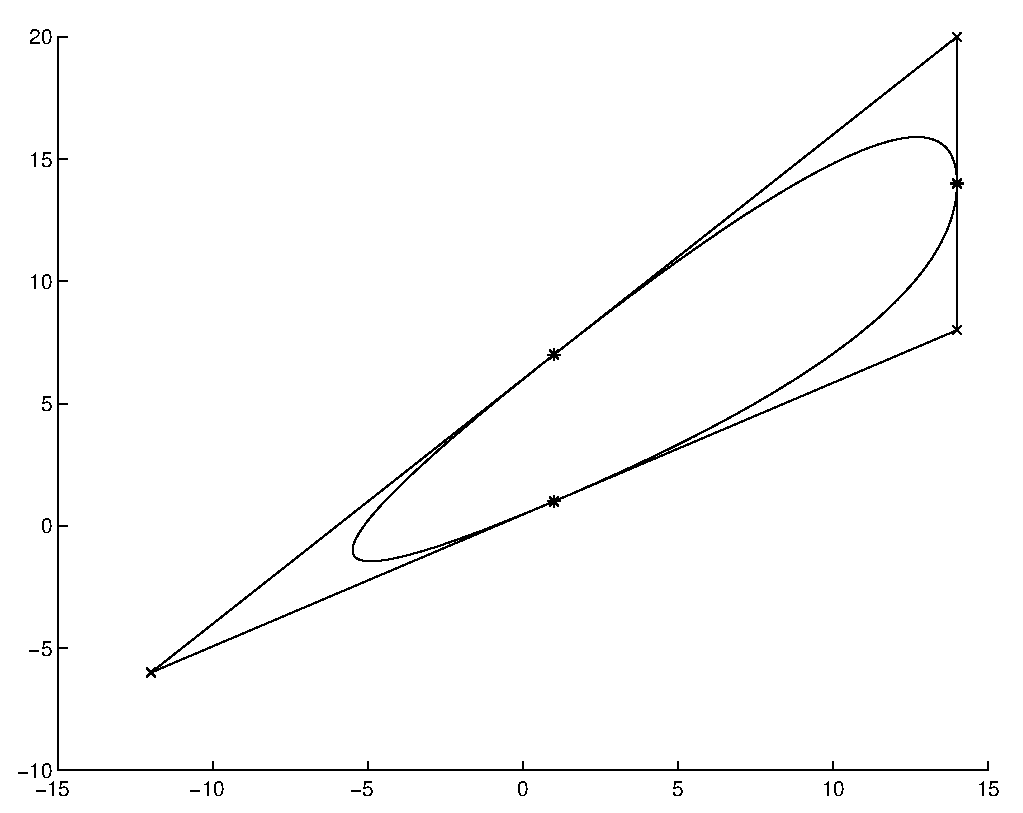
\includegraphics{eps}
  \caption{Example $\mathbf{C}_1$-continous B\'ezier spline}
\end{figure} 

\hfill
$\square$

\section*{Task 4.4: Chaikin's Corner Cutting}

\section*{Task 4.5: Bilinear Surfaces}

We can use the formula for the Linear B\'ezier curve

$$B(t) = (1-t)P_0 + tP_1, \quad 0 \leq t \leq 1$$

where points $P_i$, $i=0,1$ are the corners of the provided surface ($b_{ij}$,
$i,j=0,1$) that we are interpolating between. We first interpolate between
($b_{00}$, $b_{01}$), and ($b_{01}$, $b_{11}$). We can then interpolate between
the obtained points to get the answer.

\begin{align*}
  b_{00} &= \Spvek{0;0;0}, \quad b_{10} = \Spvek{1;0;1}, \quad b_{01} = \Spvek{0;1;1}, \quad b_{11} = \Spvek{1;1;0}\\
  \pmb{x}(\frac{1}{2}, 0) 	    &= \frac{1}{2}b_{00} + \frac{1}{2}b_{10} = \Spvek{\frac{1}{2};0;\frac{1}{2}}\\
  \pmb{x}(\frac{1}{2}, 1) 	    &= \frac{1}{2}b_{01} + \frac{1}{2}b_{11} = \Spvek{\frac{1}{2};1;\frac{1}{2}}\\
  \pmb{x}(\frac{1}{2}, \frac{1}{2}) &= \frac{1}{2}\pmb{x}(\frac{1}{2}, 0) + \frac{1}{2}\pmb{x}(\frac{1}{2}, 1) = \Spvek{\frac{1}{2};\frac{1}{2};\frac{1}{2}}\\
\end{align*}

\end{document}
